\Askhsh{18555_SOLUTION}{1}
\begin{ylh}{1}
    \item [Λύση ασκήσεων με τριγωνομετρία και εμβαδά.]
\end{ylh}
\begin{wrapfigure}[15]{r}{0.5\textwidth}
\centering
\begin{tikzpicture}[scale=0.8]
    % Ορισμός σημείων με βάση τις υπολογιστικές παραδοχές:
    % A=(0,0), B=(alpha,0), Sigma=(2*alpha,0), Delta=(0,alpha), Gamma=(alpha,alpha)
    % Για την σχεδίαση, θέτουμε alpha = 2 μονάδες.
    \tkzDefPoint(0,0){A}
    \tkzDefPoint(2,0){B} % B βρίσκεται στην απόσταση alpha από το A
    \tkzDefPoint(4,0){Sigma} % Sigma βρίσκεται στην απόσταση alpha από το B, οπότε 2*alpha από το A
    \tkzDefPoint(6,0){SigmaPrime} % SigmaPrime βρίσκεται δεξιότερα του Sigma
    \tkzDefPoint(0,2){Delta} % Delta βρίσκεται σε ύψος alpha από το A
    \tkzDefPoint(2,2){Gamma} % Gamma βρίσκεται σε ύψος alpha από το B και στην ίδια γραμμή με το Delta

    % Σχεδίαση της κύριας οριζόντιας γραμμής (βάση)
    \tkzDrawLine[add=0 and 0.5, thick, color=black](A,SigmaPrime)

    % Σχεδίαση των κατακόρυφων γραμμών από το A στο Delta και από το B στο Gamma
    \tkzDrawSegment[thick, color=black](A,Delta)
    \tkzDrawSegment[thick, color=black](B,Gamma)

    % Σχεδίαση των τμημάτων για το τρίγωνο DeltaGammaSigma (χρώμα maincolor)
    \tkzDrawSegment[thick, color=maincolor](Delta,Sigma)
    \tkzDrawSegment[thick, color=maincolor](Gamma,Sigma)

    % Σχεδίαση των τμημάτων για το τρίγωνο DeltaGammaSigmaPrime (χρώμα secondarycolor)
    \tkzDrawSegment[thick, color=secondarycolor](Delta,SigmaPrime)
    \tkzDrawSegment[thick, color=secondarycolor](Gamma,SigmaPrime)

    % Τοποθέτηση ετικετών για τα σημεία
    \tkzLabelPoint[below](A){A}
    \tkzLabelPoint[below](B){B}
    \tkzLabelPoint[below](Sigma){$\Sigma$}
    \tkzLabelPoint[below](SigmaPrime){$\Sigma'$}
    \tkzLabelPoint[above left](Delta){$\Delta$}
    \tkzLabelPoint[above right](Gamma){$\Gamma$}

    % Τοποθέτηση ετικέτας για το ύψος alpha
    \tkzLabelSegment[left](Delta,A){$\alpha$}
\end{tikzpicture}
\end{wrapfigure}
\begin{alist}
\item [\textalpha)]
  Για το εμβαδό του τριγώνου $\Delta\Gamma\Sigma$ μπορούμε να πάρουμε για βάση την πλευρά $\Delta\Gamma$ και για ύψος την κάθετη από το $\Sigma$ προς τη $\Delta\Gamma$, η οποία είναι ίση με $\alpha$, οπότε $\left(\Delta\Gamma\Sigma\right) = \frac{\alpha \cdot \alpha}{2} = \frac{\alpha^2}{2}$, δηλαδή ισούται με το μισό του εμβαδού του αρχικού τετραγώνου. \monades{X}
\begin{rlist}
\item [i.]
  Για να υπολογίσουμε την περίμετρο του τριγώνου $\Sigma\Delta\Gamma$ θα χρειαστεί να υπολογίσουμε τα μήκη των πλευρών του $\Sigma\Delta$ και $\Sigma\Gamma$ ως συνάρτηση του $\alpha$.
  Από το Πυθαγόρειο θεώρημα στο τρίγωνο $\Sigma B\Gamma$ έχουμε $\Sigma\Gamma^2 = \Sigma B^2 + B\Gamma^2$ ή $\Sigma\Gamma^2 = \alpha^2 + \alpha^2$ ή $\Sigma\Gamma^2 = 2\alpha^2$ ή $\Sigma\Gamma = \alpha\sqrt{2}$.
  Αντίστοιχα από το Πυθαγόρειο θεώρημα στο τρίγωνο $A\Sigma\Delta$ έχουμε $\Sigma\Delta^2 = \Sigma A^2 + A\Delta^2$ ή $\Sigma\Delta^2 = \left(2\alpha\right)^2 + \alpha^2$ ή $\Sigma\Delta^2 = 5\alpha^2$ ή $\Sigma\Delta = \alpha\sqrt{5}$.
  Οπότε η περίμετρος του τριγώνου $\Sigma\Delta\Gamma$ είναι ίση με $\Sigma\Gamma + \Sigma\Delta + \Delta\Gamma = \alpha\sqrt{2} + \alpha\sqrt{5} + \alpha$. \monades{X}
\end{rlist}
\item [\textbeta)]
  Τα τρίγωνα $\Sigma\Delta\Gamma$ και $\Sigma'\Delta\Gamma$ έχουν κοινή πλευρά τη $\Delta\Gamma$ οπότε ο λόγος των εμβαδών τους ισούται με το λόγο των αντίστοιχων υψών τους προς την πλευρά αυτή.
  Όμως τα ύψη αυτά εκφράζουν την απόσταση των παραλλήλων πλευρών του τετραγώνου, οπότε είναι ίσα μεταξύ τους και ίσα με την πλευρά $\alpha$ του τετραγώνου.
  Άρα $\frac{\left(\Sigma\Delta\Gamma\right)}{\left(\Sigma'\Delta\Gamma\right)} = \frac{\alpha}{\alpha} = 1$, οπότε τα εμβαδά των τριγώνων $\Sigma\Delta\Gamma$ και $\Sigma'\Delta\Gamma$ είναι ίσα μεταξύ τους και το καθένα ίσο με το μισό του εμβαδού του τετραγώνου, όπως φαίνεται στο \textalpha)\text{i)}.
  Συνεπώς ο ισχυρισμός του Βρασίδα σχετικά με τα εμβαδά των δύο τριγώνων δεν είναι σωστός.
  Το τρίγωνο $\Sigma'\Delta\Gamma$ είναι ισεμβαδικό με το τρίγωνο $\Sigma\Delta\Gamma$. \monades{X}
\begin{rlist}
\item [ii.]
  Σύμφωνα με αυτό που αποδείχθηκε στην τάξη ισχύει ότι: $\Sigma'\Gamma > \Sigma\Gamma$ και $\Sigma'\Delta > \Sigma\Delta$, άρα, $\Delta\Gamma + \Sigma'\Gamma + \Sigma'\Delta > \Delta\Gamma + \Sigma\Gamma + \Sigma\Delta$, οπότε η περίμετρος του τριγώνου $\Sigma'\Delta\Gamma$ είναι μεγαλύτερη από την περίμετρο του τριγώνου $\Sigma\Delta\Gamma$.
  Ο ισχυρισμός του Βρασίδα για τις περιμέτρους των δύο τριγώνων είναι σωστός. \monades{X}
\end{rlist}
\end{alist}